\subsection{Stream Partitioning}
We use the Geohash~algorithm~\cite{geohash} to balance load and partition incoming data streams across processing resources. Geohash divides the earth into a hierarchy of bounding boxes identified by Base 32 strings; the longer the Geohash string, the more precise the bounding box. Figure~\ref{fig:geohash} illustrates this hierarchy. Most of the eastern United States is contained within the bounding box described by Geohash string \emph{D}, while \emph{DJ} encompasses substantial parts of Florida, Georgia, and Alabama. The bounding box \emph{DJKJ} (highlighted in red) contains Tallahassee, Florida. This hierarchical representation enables \textsc{Synopsis} to cope with both low- and high-density regions: several resources may be tasked with managing streams originating in and around large cities, while rural areas fall under the purview of a single node.

\begin{figure}
    \centerline{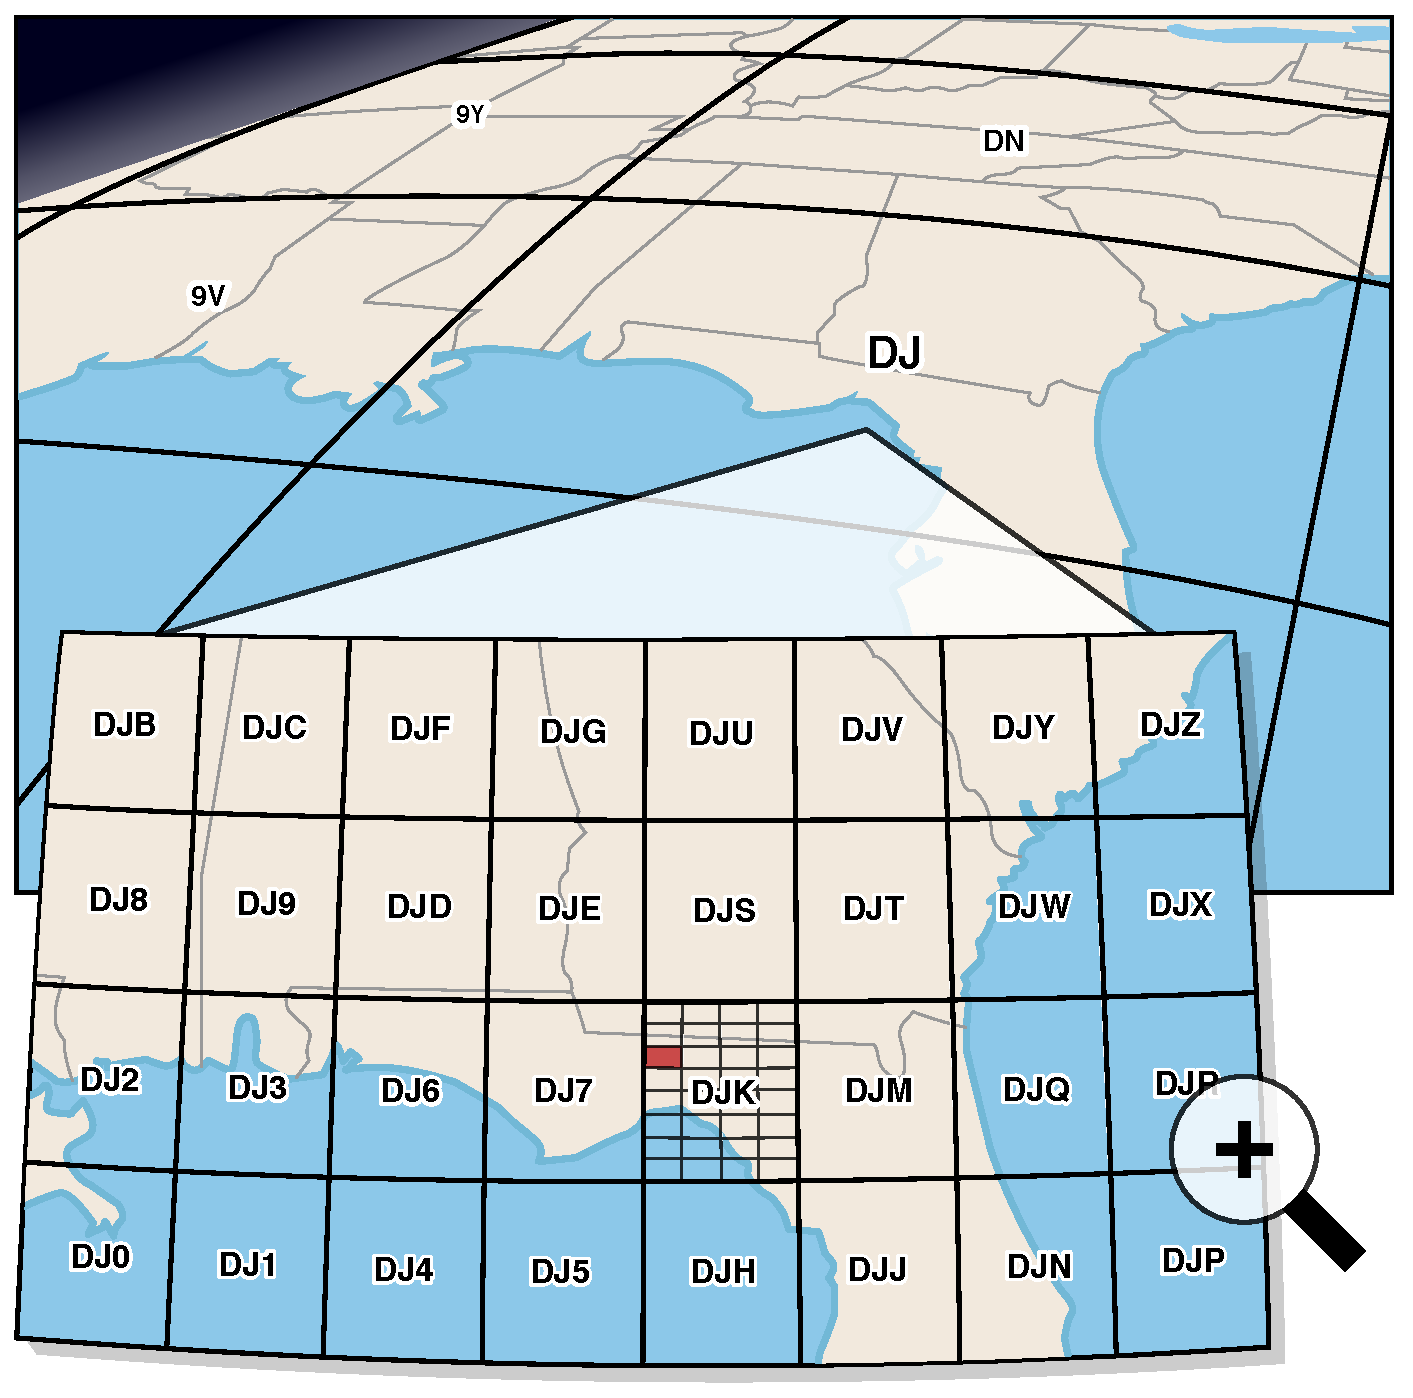
\includegraphics[width=3.5in]{figures/geohash.pdf}}
    \caption{A demonstration of the Geohash algorithm. Each additional character in a Geohash string describes a finer-grained region; Geohash \emph{DJ} contains substantial parts of Florida, Georgia, and Alabama, USA, while \emph{DJKJ} (highlighted in red) encompasses Tallahassee, the capital of Florida.}
    \label{fig:geohash}
\end{figure}

To achieve fine-grained control over our Geohash partitions, we operate at the bit level rather than Base 32 character level when routing streams. Each bit added to a Geohash string reduces its scope by half, with each character represented by five bits ($2^5 = 32$). In other words, a four-character Geohash string represents 20 spatial subdivisions. This property allows us to manage and allocate resources across a wide variety of observational densities.

Figure~\ref{fig:stream-partitioning} depicts a possible arrangement of the distributed sketch and the associated stream partitioning scheme corresponding to the same geographic region described above.
The distributed sketch is arranged in a tree-like structure.
Stream ingesters act as root nodes of this tree structure and they partition the geo-spatial stream among the \textsc{Synopsis} nodes using the Geohash based partitioning function.
Nodes closer to the root hold sketches corresponding to shorter Geohash strings.
In other words, they contain sketches for larger geographical regions.
For instance, nodes A and B in Figure~\ref{fig:stream-partitioning} are responsible for regions represented by Geohashes \emph{DJ} and and \emph{DN} respectively.
Node E, which is 3 edges deep from the stream ingester, is responsible for a smaller region, \emph{DJKJ}.

\textsc{Synopsis} is designed to ensure that the regions which are corresponding to larger portions of input streams, hence more frequent updates to the sketch, are moved to dedicated or less crowded nodes.
If a node decides to scale out a portion of the region it is currently responsible for, then the corresponding state (sketch and related meta data) is transferred over to the new computation and it starts to treat the stream packets corresponding to the scaled out region as pass-through traffic (Scaling out is explained in section~\ref{subsec:scaling-out}).
More specifically, it will not process the stream packet, instead updates its statistics based on the headers of the packet and forwards it to the child node . 
For instance, node A in Figure~\ref{fig:stream-partitioning} have scaled out two regions (\emph{DJK} and \emph{DJM}) to nodes C and D.
After these two scaling out operations, node A is responsible for all sub-regions in \emph{DJ} except for \emph{DJK} and \emph{DJM}.
Similarly the sketch for the region \emph{DJKJ} is moved out of node C into node E as a result of subsequent scale out operation.
It should be noted that the depth and span of the distributed sketch are dynamic and are constantly evolving according to the workload and operating conditions.

When the height of the tree grows, it becomes inefficient to have parent nodes passing through the traffic intended for the child nodes. 
Because it consumes extra bandwidth as well as increases the latency of the  corresponding sketch updates due to increased number of hops the packets have to travel through.
To circumvent this, we use short circuiting to direct traffic from stream ingesters straight to child nodes and avoid routing through parents.
This is depicted in Figure~\ref{fig:stream-partitioning} where stream ingester directly sends data to node E instead of sending it through nodes A and C.
We use our gossiping subsystem to update parents on the statistics related to child prefixes which are useful for scaling in decisions at later points of time as explained in section~\ref{subsec:scaling-out}.
Due to short circuiting, the data flow path starts to deviate from the tree like structure of the distributed sketch.

\begin{figure}
    \centerline{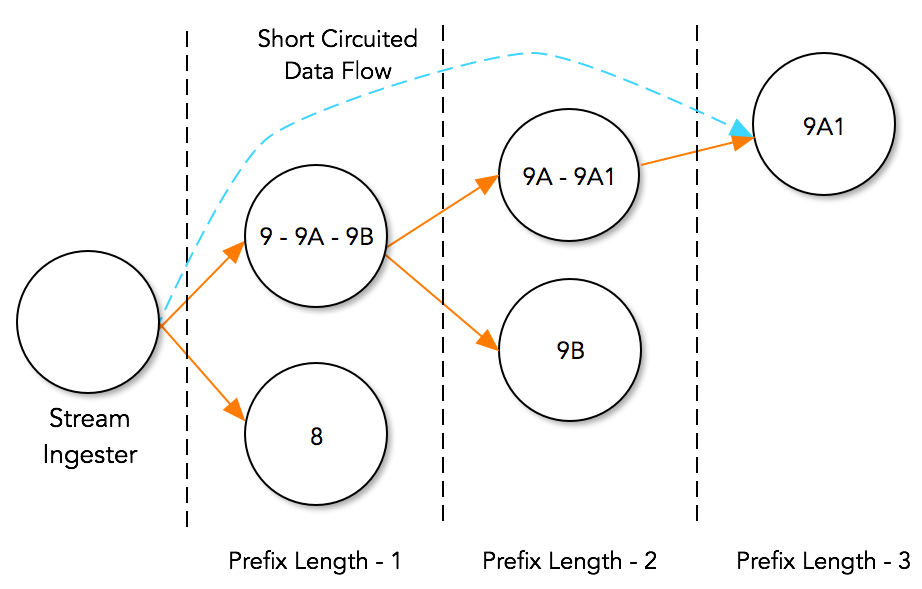
\includegraphics[width=3.5in]{figures/stream-partitioning.png}}
    \caption{An example of the stream partitioning based on Geohashes of the stream packets}
    \label{fig:stream-partitioning}
\end{figure}
